\section{Module 1: Lectures 1 - 3}


\subsection{Introduction}
With the advent of the internet, the amount of audio, video and image data has gone up. Processing this data for efficient storage and for a better human experience of them is a must. Apart from these types of data, there has also been a rise in data as describing the history of some phenomenon as a result of the numerous scientific experiments conducted and the world of financial markets. Data describing the temperature variation over a region, data describing the variation in the price of a stock over time are examples. It is imperative to process this kind of data in order to infer from it. A very important characteristic of this kind of data is that it can be described as a function of a variable - discrete or continuous. We can think of this data as a signal. And to process these varied types of signals, we construct systems. And it is these systems that we plan to learn about in this course. Below, we start with an introduction to abstraction, a process fundamental to the study of signals and systems.

\subsection{Abstractions}
The process of extracting out common attributes by doing away with the situation specific details irrelevant to the purpose at hand, from apparently different situations, is abstraction. The process of abstraction aids us by reducing our work as we can then conduct a study of all the situations all at once. It also provides us with an opportunity to apply insights from one specific situation to the others. All this is demonstrated by the example below.

We consider a mass $m$ and a capacitor $C$. Let $F(t)$ be the force acting on the mass and let $v(t)$ be its velocity. From Newton's second law,
\[
F(t) = m\frac{dv(t)}{dt}
\]

In the case of the capacitor, if $i(t)$ is the current flowing through the capacitor and $v_{C}(t)$ is the voltage across it, then we know,
\[
i(t) = C\frac{dv_{C}(t)}{dt}
\]

We first notice that both of these are systems. The force $F(t)$ and the current $i(t)$ are the input signals to these systems and the velocity $v(t)$ and the voltage $v_{C}(t)$ are the corresponding output signals.

If one looks at the above relations carefully, one cannot help
but notice the striking similarity between the two. If we consider the
force $F(t)$, the mass $m$ and the velocity $v(t)$ of the mass to be
analogous to the current $i(t)$, the capacitor $C$ and the voltage
across the capacitor $v_{C}(t)$ respectively , the relations are the same. Now, we can just solve this one differential equation, forgetting conveniently the mass and the capacitor, and hence obtain the behaviour of both these systems at the same time. This is the power of abstraction.\\

Consider now, a viscous force proportional to the velocity of the mass with $\kappa_{0}$ being the constant of proportionality.\footnote{This is an approximation that is reasonably accurate at low velocities of the mass.} The force $F(t)$ now has to also overcome the opposing viscous force. Fig. 1(a) illustrates the situation. In the case of the mass, the equation describing the system now becomes,
\[
F(t) = m\frac{dv(t)}{dt} + \kappa_{0}v(t)
\]

Also, consider a resistance $R$ in series with the capacitor considered above. The circuit diagram is shown in fig. 1(b). For the RC circuit, the current flowing through the resistance is $C\frac{dv_{C}(t)}{dt}$, equal to the current flowing through the capacitor. By Kirchoff's law, $v_{in}(t)$ is equal to the sum of the voltages across the resistance and the capacitor. Thus,
\[
v_{in}(t) = v_{C}(t) + RC\frac{dv_{C}(t)}{dt}
\]
Dividing both sides by $R$,
\[
\frac{1}{R}v_{in}(t) = C\frac{dv_{C}(t)}{dt} + \frac{1}{R}v_{C}(t)
\]

Again, there is a striking similarity between this relation and the relation for the mass system. Thus, it is clear that the two systems considered above are very similar in their behaviour.

%http://en.wikipedia.org/wiki/RC_circuit#mediaviewer/File:RC_Series_Filter_(with_V%26I_Labels).svg 
\begin{figure}[H]
        \centering
        \begin{subfigure}[b]{0.4\textwidth}
                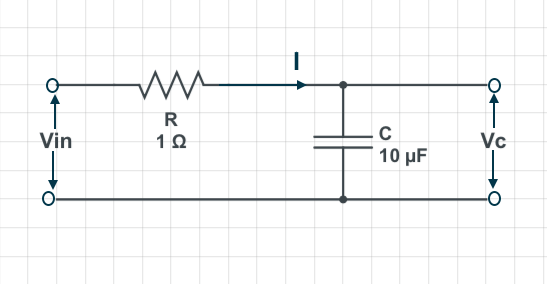
\includegraphics[width=\textwidth]{my_rc.png}
                \caption{An RC series circuit}
        \end{subfigure}
        \quad
	~
        \begin{subfigure}[b]{0.5\textwidth}
                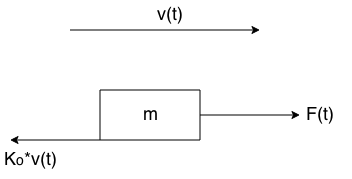
\includegraphics[width=\textwidth]{fbd.png}
                \caption{Forces acting on the mass}
        \end{subfigure}
        \caption{}
\end{figure}


\subsection{Definitions}
\subsubsection{Signal}
A signal is a ``reasonable" function of a real independent variable to the set of complex numbers in the most general case. Thus a function $x(t)$ is a signal if $x:\mathbb{R} \xrightarrow{} \mathbb{C}$ \footnote{The definition given here defines a signal with one dimensional independant and dependant variables. However signals with multidimensional independant variables are quite common as well. An image is an example with a two dimensional independant variable.} and $x(t)$ is reasonable. By reasonable, here we mean that the function should be well-behaved and hence, often something we may encounter practically. For example, the Dirichlet function $I_{Q}$ defined below is unreasonable in the sense that it is continuous nowhere on its domain and it is very improbable that this function will be encountered practically. Hence we do not consider this a signal.
\[
I_{Q}(x) =
  \begin{cases}
      \hfill 1 \hfill & \text{ if $x$ is rational} \\
      \hfill 0 \hfill & \text{ if $x$ is irrational} \\
  \end{cases}
\]

A signal is defined above to be a mapping to the set of complex numbers. The reason to consider a mapping to complex numbers is not yet clear as all the examples we have considered were real valued. However, we note that the definition given is a more general one as the set of reals is a subset of the set complex numbers. The reason for this generality will become clear as we go further in the course.\\

A couple of examples of signals are given in fig. 2 below.

%http://seismo.berkeley.edu/blog/seismoblog.php/2008/09/10/p-waves-and-s-waves-which-are-faster

\begin{figure}[H]
        \centering
        \begin{subfigure}[b]{\textwidth}
                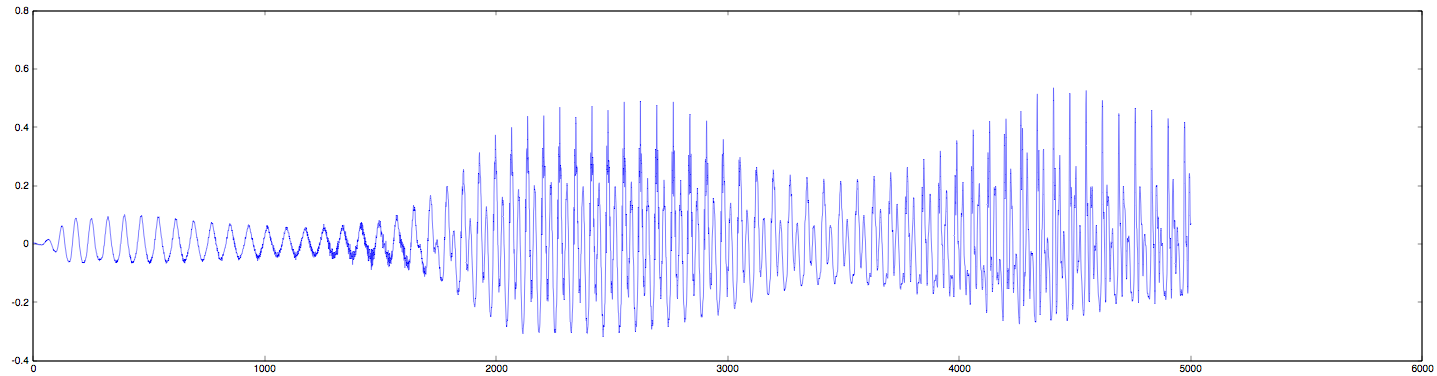
\includegraphics[width=\textwidth]{signal1_hello.png}
                \caption{An Audio Signal}
        \end{subfigure}
        \quad
        ~ %add desired spacing between images, e. g. ~, \quad, \qquad, \hfill etc.
          %(or a blank line to force the subfigure onto a new line)
        \centering
        \begin{subfigure}[b]{0.5\textwidth}
                
\includegraphics[width=\textwidth]{signal2_lena.png}
                \caption{An image: A 2D Signal}
        \end{subfigure}
        \caption{}
\end{figure}

\subsubsection{System}
A system is a mapping from a set of signals to another set of signals. A system thus takes a signal as an input and returns another signal as its output. A microphone is an example of a system. This system is a mapping from the set of acoustic signals to a set of electric signals.

\subsubsection{System Description}
Given a system, a system description is an explicit or an implicit relation between the inputs and the outputs of the system. By an implicit relation, we mean a relation of the form $F(x(t), y(t)) = 0$ where F is a function of two signals, the input signal $x(t)$ and the output signal $y(t)$. Thus it is not always possible to directly compute $y(t)$ directly in terms of $x(t)$. Description \textit{1} given below is an explicit system description while description \textit{2} is an implicit one.
\begin{enumerate}
\item[\textit{1}] $y(t) = x(t) + 3\frac{dx(t)}{dt}$
\item[\textit{2}] $y(t)x(t) + x(t)\frac{dy(t)}{dt} = 0$
\end{enumerate}

\subsection{Properties of Systems}
Given a system description, a lot can be inferred about the system. We describe below some properties that systems may or may not possess and give examples of each. These properties aid in the further study and classification of systems.

\subsubsection{Additivity}
A system $S$ is said to be additive if for any two input signals $x_{1}(t)$ and $x_{2}(t)$,
\[
x_{1}(t) \xrightarrow{S} y_{1}(t) \; and \; x_{2}(t) \xrightarrow{S} y_{2}(t)
\]
\begin{center}
imply
\end{center}
\[
x_{1}(t) + x_{1}(t) \xrightarrow{S} y_{1}(t) + y_{2}(t)
\]

The systems $y(t) = 3x(t)$ and $\frac{dy(t)}{dt} = x(t)$ are both additive while the system $y(t) = x(t) + 4$ (a DC shift in the case of electrical signals) is not because of the constant.

\subsubsection{Homogeneity}
A system $S$ is said to be homogenous if for every input signal $x(t)$ and for every $c \in \mathbb{C}$,
\[
x(t) \xrightarrow{S} y(t)
\]
\begin{center}
implies
\end{center}
\[
cx(t) \xrightarrow{S} cy(t)
\]

This property is also referred to as the scaling property.\\

The systems $y(t) = 3x(t)$ and $\frac{dy(t)}{dt} = x(t)$ are both homogeneous too while the system $y(t) = x(t) + 4$ is non-homogeneous again due to the presence of the non zero constant.

\subsubsection{Shift Invariance}
A system S is said to be shift invariant if for all input signals $x(t)$ and for every $t_{0} \in \mathbb{R}$,

\[
x(t) \xrightarrow{S} y(t)
\]
\begin{center}
implies
\end{center}
\[
x(t - t_{0}) \xrightarrow{S} y(t - t_{0})
\]

Intuitively, the property of shift invariance implies that if the same input is fed to the system at different times, then the output of the system will only be shifted in time by the same amount 
as that of the input.

Thus, the system $y(t) = x(t^{2})$ is shift invariant while the system $y(t) = tx(t)$ is not.\\
\textbf{Note:} The property of shift invariance is also referred to by many as time invariance.

\subsection*{Some Additional Material}
\subsubsection{Abstraction}
As the professor alludes to in the video segment, the process of abstraction is the most important tool we use for analysing and studying the natural world. A very good example of abstraction is the theory of gravitation. The insight that an apple falling from the tree (and supposedly hitting his head) and the Moon revolving around the Earth are actually the same thing was something only Newton could have had. In his words, ``....I began to think of gravity extending to the orb of the Moon....''. At that moment in history, he abstracted out all the differences between the moon and the apple to come up with the theory of universal gravitation. The word universal in the name is important as it states how we can think of (i.e abstract) every mass in the Universe as a point mass attracting every other. That is the power of abstraction as the instructor stresses in the video segment.

However one must keep in mind that the real art lies in finding the right kind and the right level of abstraction for the specific kind of job at hand. Suppose a chemist wants to study chemical behaviour of ethanol and methanol in connection with their reactions with some particular chemical. In that case, abstracting out the fact whether it is methyl or ethyl alcohol and studying, in generality the reactions of the alcohol part of the two (i.e. of the -OH group) with the desired chemical considerably reduces the work of the chemist. However, we cannot use the same abstraction when studying the biological effects of the two as methanol is highly toxic and can be fatal in sufficient quantities; however ethanol is not toxic and is used for....well we all know!


